\section{جمع‌بندی و نتیجه‌گیری}
\label{sec:conclusion}

% در این پایان‌نامه، طراحی و پیاده‌سازی سامانه‌های غیرتماسی پایش علائم حیاتی مبتنی بر رادار \lr{FMCW} بررسی شد. مهم‌ترین نتایج به‌صورت زیر خلاصه می‌شوند:

% \begin{enumerate}
%     \item \textbf{تعیین برتری معماری \lr{FMCW}:}
%     \begin{itemize}
%         \item رادارهای \lr{FMCW} توازن مناسبی بین پیچیدگی سخت‌افزاری و قابلیت‌های فاصله‌یابی و تفکیک چندهدفه ارائه می‌دهند، در حالی که \lr{CW} از نظر سخت‌افزار ساده بوده اما در برابر کلاتر محیطی آسیب‌پذیر است و \lr{UWB} با وجود دقت بالا نیازمند سخت‌افزار و پردازش پیشرفته است.
%         \item تحلیل داده‌های تجربی نشان داد که معماری \lr{FMCW} پایین‌ترین میانه‌ی خطای مطلق ($\mathrm{MAE} < 2\ \mathrm{bpm}$) در اندازه‌گیری ضربان قلب را ثبت کرده است و توزیع خطاهای آن فشرده‌تر از دو معماری دیگر است.
%     \end{itemize}

%     \item \textbf{انتخاب بهینه فرکانس و پهنای باند:}
%     \begin{itemize}
%         \item پهنای باند در محدوده‌ی \lr{1–4 GHz}، رزولوشن فاصله‌ای زیرسانتی‌متری را برای کاربردهای پزشکی در برد عملیاتی \lr{0.5–3 m} فراهم می‌کند.
%         \item فرکانس‌های حامل میانی (\lr{60–80 GHz}) به دلیل حساسیت فاز مناسب و عمق نفوذ کافی، بهترین گزینه برای سامانه‌های پوشیدنی و بالینی هستند؛ فرکانس‌های بالاتر تا \lr{120 GHz} دقت بیشتری ارائه می‌دهند اما پیچیدگی آنتن و مصرف انرژی را افزایش می‌دهند.
%     \end{itemize}

%     \item \textbf{معماری سخت‌افزار و \lr{MIMO}:}
%     \begin{itemize}
%         \item استفاده از چیپ \lr{IWR1642} با آرایه \lr{MIMO} (۳\lr{TX}$\times$۴\lr{RX}) امکان جداسازی چندشخصه و تعیین زاویه را به‌سادگی فراهم می‌کند و وضوح زاویه‌ای حدود $16.6^\circ \times 45^\circ$ را میسر می‌سازد.
%         \item بردهای ارزیابی ماژولار مبتنی بر \lr{BGT24} و \lr{BGT60} امکان مقایسه و تنظیم سریع پارامترها را فراهم می‌کنند و مصرف توان سیستم نهایی زیر \lr{30 mW} حفظ شده است.
%     \end{itemize}

%     \item \textbf{الگوریتم‌های پردازش سیگنال:}
%     \begin{itemize}
%         \item زنجیره‌ی پردازش شامل کالیبراسیون \lr{DC}، استخراج و \lr{Unwrapping} فاز، تفاضل فاز و فیلترینگ \lr{IIR}، حذف آرتیفکت حرکتی و \lr{STFT} است که دقت \lr{HR} را تا $\mathrm{MAE} < 2\ \mathrm{bpm}$ تضمین می‌کند.
%         \item الگوریتم \lr{Health-VMD} با تابع هدف \lr{PME} و بهینه‌سازی \lr{GOA} امکان استخراج دقیق \lr{HRV} با $\mathrm{RMSE} \approx 4.1\ \mathrm{ms}$ را مهیا ساخته است، که در کاربردهای چندنفری عملکرد پایدار دارد.
%     \end{itemize}

%     \item \textbf{رعایت ایمنی و استانداردها:}
%     \begin{itemize}
%         \item توان خروجی تنظیم‌شده ($\sim$3.16 \lr{mW}) به‌طور ایمن زیر محدودیت‌های \lr{ICNIRP} و \lr{FCC} قرار دارد و \lr{SAR} کمتر از \lr{0.05 W/kg} است.
%         \item انطباق با استانداردهای \lr{IEC 60601-1-2}، \lr{IEEE 1528} و \lr{ISO 14971} فرایند ثبت \lr{FDA}، \lr{CE} و \lr{IR-MOH} را تسهیل می‌کند و خطرات تابش و تداخل به حداقل می‌رسد.
%     \end{itemize}
% \end{enumerate}

% \subsection*{چشم‌انداز آینده}
% \label{sec:future-work}

% با وجود پیشرفت‌های قابل توجه در سامانه‌های \lr{FMCW} پزشکی، فرصت‌های پژوهشی متعددی باقی است:

% \begin{itemize}
%     \item \textbf{هوش مصنوعی در پردازش بلادرنگ:} ترکیب یادگیری عمیق با مراحل پردازش می‌تواند دقت و مقاومت الگوریتم‌ها در برابر حرکت‌های تصادفی را بهبود بخشد.
%     \item \textbf{بهینه‌سازی انرژی و طراحی پوشیدنی:} تحقیق روی منابع انرژی کم‌حجم و ادغام سامانه در پوشیدنی‌های سبک (مانند ساعت هوشمند) برای نظارت مداوم بی‌وقفه.
%     \item \textbf{گسترش به علائم حیاتی دیگر:} توسعه الگوریتم‌های تحلیل سیگنال برای اندازه‌گیری فشار خون، اشباع اکسیژن و دمای پوست با استفاده از ترکیب چندحسی.
%     \item \textbf{مطالعات بالینی گسترده:} اجرای آزمون‌های چندمرکزه با جمعیت متنوع برای اعتبارسنجی نتایج در محیط‌های بالینی واقعی.
% \end{itemize}

% در نهایت، سامانه‌های \lr{FMCW} با پتانسیل تطبیق‌پذیری بالا و قابلیت ترکیب با فناوری‌های پوشیدنی، افق روشنی برای پزشکی از راه دور و مراقبت‌های هوشمند باز می‌کنند. این پایان‌نامه با ارائه یک چارچوب یکپارچه از مبانی تئوری تا پیاده‌سازی عملی، گامی مهم در جهت توسعه این فناوری برداشته است.
% \subsection*{نتیجه‌گیری}
% \label{sec:chapter3-conclusion}

فصل سوم نشان داد که معماری \lr{FMCW} می‌تواند به‌عنوان راهکاری عملی برای پایش غیرتماسی علائم حیاتی در محیط‌های بالینی و خانگی به‌کار رود. با انتخاب فرکانس حامل \lr{60 GHz} و پهنای باند \lr{1–4 GHz}، تفکیک فاصله به‌اندازه‌ی نیازهای مراقبت پزشکی تأمین می‌شود و حساسیت فاز برای آشکارسازی ریزحرکت قفسه‌ی سینه بهبود می‌یابد. مقایسه‌ی تجربی میان سامانه‌های \lr{24 GHz}، \lr{60 GHz} و \lr{120 GHz} نشان داد که بازه‌ی \lr{60–120 GHz} بهترین توازن میان عمق نفوذ، مصرف توان و دقت اندازه‌گیری را فراهم می‌کند، در حالی که سامانه‌ی \lr{24 GHz} به‌دلیل پهنای باند محدود و نویز بالاتر، عملکرد ضعیف‌تری دارد.

در سطح سخت‌افزار، استفاده از تراشه‌ی یکپارچه‌ی \lr{TI IWR1642} با آرایه‌ی \lr{MIMO}، توان مصرفی کمتر از \lr{30 mW} و ابعاد کوچک را ممکن کرده است؛ ویژگی‌هایی که سامانه را برای تجهیزات پوشیدنی و تخت بیمارستانی مناسب می‌کند. زنجیره‌ی پردازش پیشنهادی—شامل ازبین‌بردن مؤلفه‌ی \lr{DC}، بازکردن فاز، فیلترگذاری باندگذر و الگوریتم \lr{Health-VMD}—موفق شده است خطای میانگین مطلق ضربان قلب را به کمتر از \lr{2 bpm} و خطای تنفس را به زیر \lr{2 brpm} کاهش دهد؛ ارقامی که با استانداردهای نظارت بالینی مطابقت دارند.

به‌طور کلی، نتایج این فصل اثبات می‌کند که با طراحی دقیق پهنای باند، انتخاب فرکانس مناسب و بهینه‌سازی زنجیره‌ی پردازش، رادار \lr{FMCW} می‌تواند به‌عنوان یک فناوری کم‌مصرف، ایمن و دقیق برای پایش مداوم علائم حیاتی به‌کار گرفته شود. گام‌های آتی شامل یکپارچه‌سازی کامل بر روی تراشه، افزایش عمر باتری، افزودن الگوریتم‌های یادگیری ماشین برای حذف حرکت‌های بزرگ و انجام ارزیابی‌های بالینی چندمرکزی است تا مسیر تجاری‌سازی و پذیرش بالینی این فناوری هموارتر گردد.



\begin{figure}[ht]
    \centering
    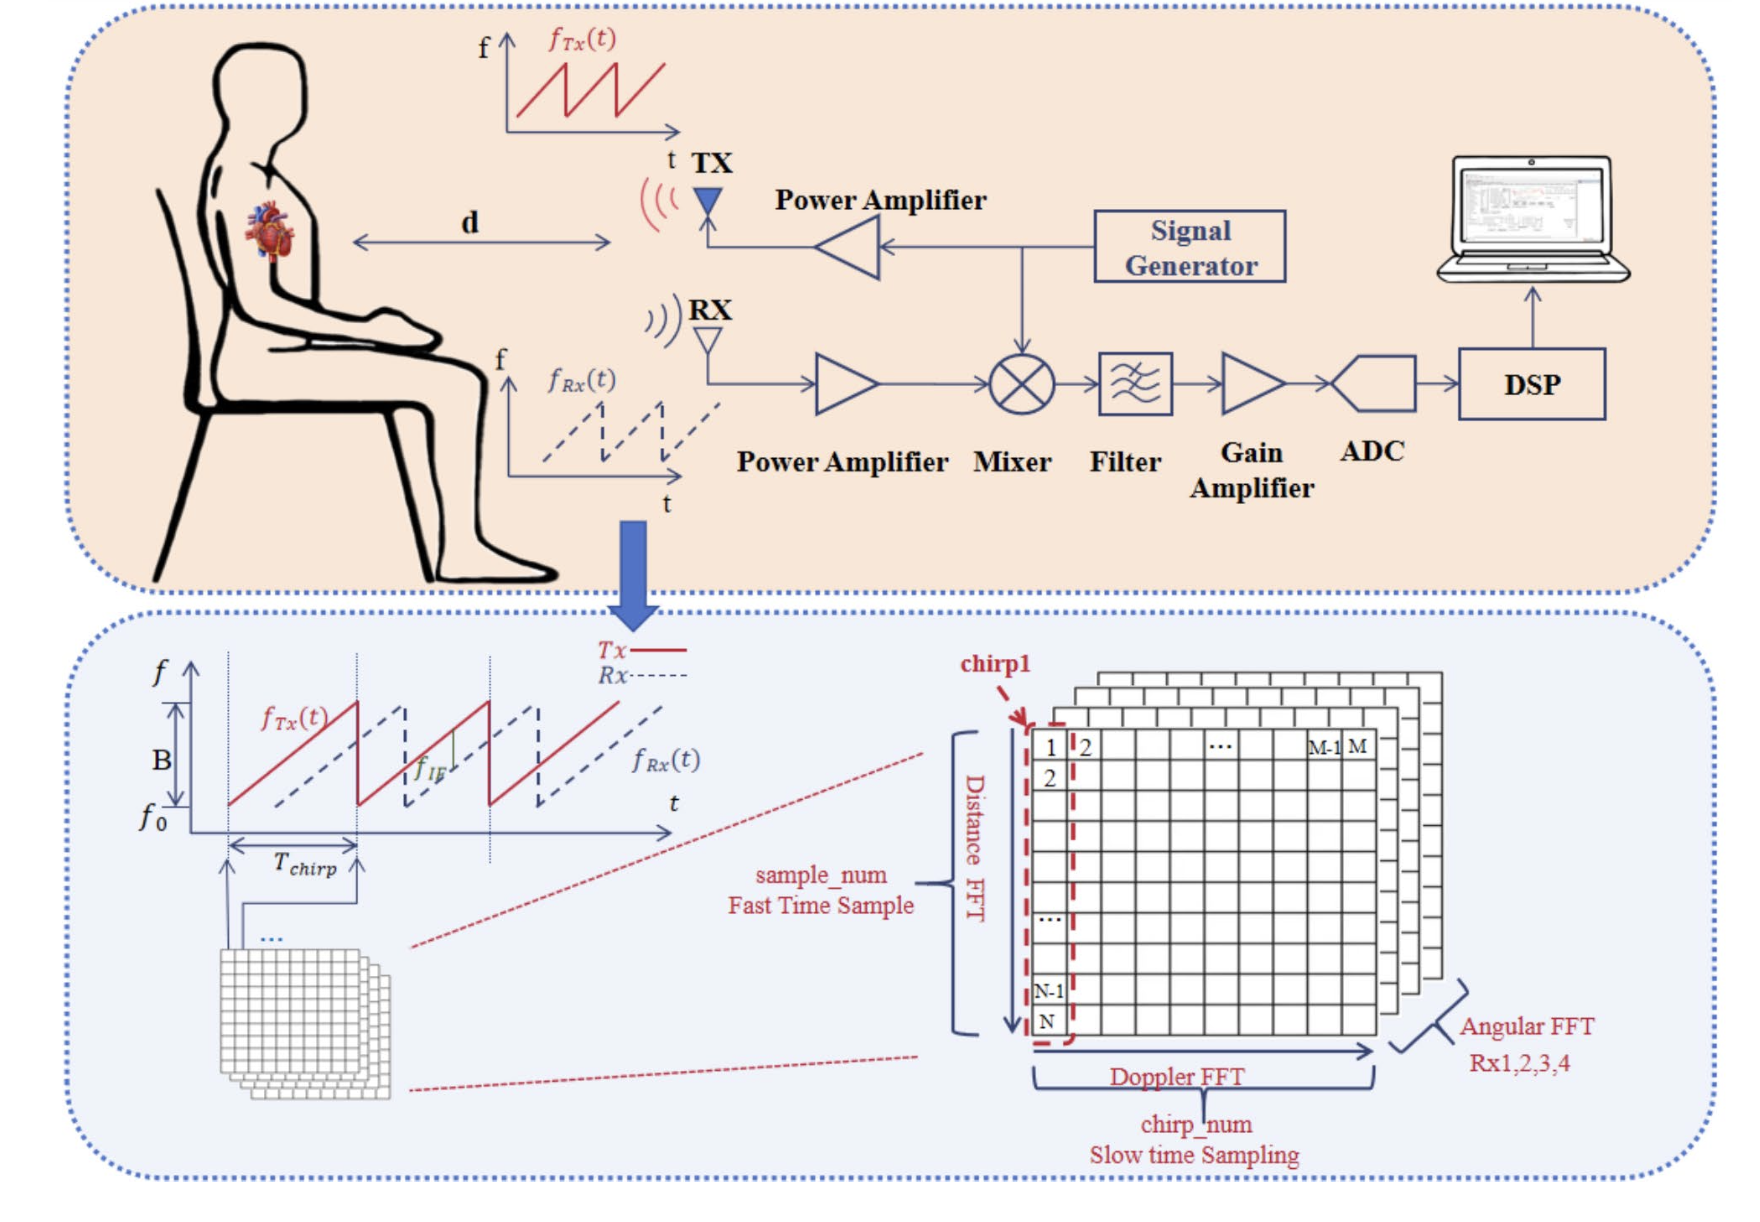
\includegraphics[width=0.7\linewidth]{Images/chapter3/3-4.png}
    \caption{
    شماتیک کلی طراحی یک سیستم تشخیص علايم حیاتی با رادار \lr{fmcw} 
    \cite{hao2025fmcw}.}
    \label{fig:fmcw_vitals}
\end{figure}